\documentclass[]{article}
%%% Document layout & text formatting
\usepackage[margin=1in]{geometry}
\usepackage[utf8]{inputenc}
\usepackage[english]{babel}

%%% Figures, tables, plots support
\usepackage{graphicx}
\usepackage{caption}
\captionsetup{justification=centering,font={small,sf}}
\usepackage{subcaption}
\usepackage{xcolor}

%%% Maths
\usepackage{amsmath}
\usepackage{amssymb}
\usepackage{wasysym}
\usepackage{siunitx}
\sisetup{separate-uncertainty = true, multi-part-units = brackets}
% fractions as powers
\usepackage{xfrac}

% differential (needs upright, not slanted d)
\newcommand{\dd}{\mathop{}\!\mathrm{d}}
% boldface vectors
\let\OLDvec\vec
\renewcommand{\vec}[1]{\boldsymbol{#1}}
% some constants
\newcommand{\rhoCentre}{\rho_\mathrm{c}}
\newcommand{\fermiMtm}{p_\mathrm{F}}
\newcommand{\massElectron}{m_\mathrm{e}}
\newcommand{\massProton}{m_\mathrm{p}}
\newcommand{\gravconst}{\mathrm{G}}


%%% References
% bibliography
%\usepackage{bibtex}
\usepackage[square,sort,comma,numbers]{natbib}
\setcitestyle{authoryear,open={(},close={)}}
\let\OLDthebibliography\thebibliography
\renewcommand\thebibliography[1]{
  \OLDthebibliography{#1}
  \setlength{\parskip}{3pt}
  \setlength{\itemsep}{0pt plus 0.3ex}
}

% hyperlinks
\usepackage{hyperref}
\hypersetup{
	colorlinks=true,
	linkcolor=blue,
	filecolor=magenta,
	urlcolor=cyan,
	citecolor=blue,
}
% more options on https://www.overleaf.com/learn/latex/hyperlinks

%%% Other new commands
% names of runs
\newcommand{\eulerOne}{\textsc{Euler1}}
\newcommand{\eulerTwo}{\textsc{Euler2}}
\newcommand{\heun}{\textsc{Heun}}
\newcommand{\rkFour}{\textsc{RK4}}

\begin{document}

% \title{This is a title}
% \author{Lyubomir Shoylev, \texttt{shil5377}}

% \maketitle

\begin{center}
	\Large{\textbf{CO31: Structure of white dwarf stars}\\
	\vspace{1em}
	\large{Lyubomir Shoylev, \texttt{shil5377}}\\ \href{mailto:me@example.com}{\texttt{lyubomir.shoylev@st-hildas.ox.ac.uk}}}\\
	\large{St Hilda's College}\\
	\today
\end{center}

\begin{abstract}
	This will be the abstract of the report. It shall be written when the rest is nearly done.
\end{abstract}

\section{Introduction}
	In this experiment the goal is to study the internal structure of white dwarf stars. They are one possible end state in the life cycle of stars. What is particular about white dwarf stars is that the matter they are composed of is different to the matter in a usual star similar to the Sun. While in a usual stable star the equilibrium is supported by fusion energy and the pressure of the plasma, a white dwarf star has exhausted its fuel and the equilibrium is supported by electron degeneracy pressure, making the star extremely dense; for example, a white dwarf of 1 solar mass is about the size of Earth. In this report, we will first derive the coupled differential equations for mass and density in a spirit similar to \cite{OxfPhys2020} and \cite{Chandrasekhar1984} in Section \ref{sec:theroy-white-dwarfs}. Then, in Section \ref{sec:numerical-approach} we develop the numerical method used to solve the coupled equations. Results and discussion take place in Section \ref{sec:results-and-discussion}. Finally, we give a summary of the experiment and possible improvements in Section \ref{sec:summary}.
	%======================= decide if the last sentence is ok

\section{Theory of white dwarf stars}\label{sec:theroy-white-dwarfs}
	Stars are astronomical objects with spherous shape made up of heated plasma. The force of gravity tries to compress the ball, holding the matter together, while the gaseous plasma opposes gravity with the pressure it exerts. When the two forces balance eachother out, the star is in hydrostatic equilibrium. In usual stars, pressure is due to the gas and due to the radiation (important mostly in the largest non-degenerate stars). In white dwarf stars however, the densities are far greater than the ones found in ususal stars, and matter behaves differently. All electrons are no longer bound to atoms and are free to roam. The behaviour is approximately described by a Fermi gas of electrons at zero Kelvin (i.e. fully degenerate state) and the pressure giving the equilibrium is the degeneracy pressure of the electrons.
	% OLD - Stars usually are spherous objects of plasma, which are held together by gravity. While gravity tries to compress the ball into a smaller size, the gaseous plasma opposes this force with the pressure it exerts. When the two forces balance eachother out the star is in equilibrium. In traditional stars, the pressure is hydrostatic (i.e. due to the high density of the gas) or radiative (from energy radiated away). In white dwarf stars however, the densities are far greater than the ones in usual stars, and matter behaves differently. All electrons are no longer bound to atoms and are free to roam. This behaviour is approximatelly decribed by a Fermi gas of electrons at zero Kelvin (i.e. fully degenerate state).
	% TODO more context about white dwarfs as evolutionary states of massive stars.

\subsection{Equation of equilibrium}\label{subsec:test}
	%		- Equation of equilibrium
	Assume the star is spherically symmetric, in equilibrium, non-rotating and the effect of magnetic fields is negligible. Therefore, all properties depend only on the distance to the centre of the star, $r$. The gravitational force on a small volume of matter with area $\dd A$ and radial height $\dd r$ is:
	\begin{equation}
		F_\mathrm{G} = - \frac{G m\left(r\right) \dd m}{r^2},
	\end{equation}
	where $m\left(r\right)$ is the mass of the star contained up to $r$, $\dd m = \dd A \dd r \rho \left(r\right)$ is the mass of the small volume and the density $\rho \left(r\right)$ was assumed constant (negative sign because it pulls towards the centre). The force due to the pressure is the difference of the forces at $r$ and $r + \dd r$:
	\begin{equation}
	F_\mathrm{P} = \left( P\left(r\right) - P\left(r + \dd r\right)\right) \dd A.
	\end{equation}
	For a star in equilibrium the two forces balance eachother out, i.e. $F_\mathrm{G} + F_\mathrm{P} = 0$. After rearranging, we get:
	\begin{equation} \label{eqn:hydrostat-equil}
		\frac{\dd P(r)}{\dd r} = \frac{P\left(r + \dd r\right) - P\left(r\right)}{\dd r} = - \frac{G \rho(r) m(r)}{r^2}.
	\end{equation}
	We can rewrite the hydrostatic equilibrium by using the chain rule:
	\begin{equation}
		\frac{\dd P(r)}{\dd r} = \frac{\dd P}{\dd \rho} \frac{\dd \rho}{\dd r},
	\end{equation}
	so equation \eqref{eqn:hydrostat-equil} becomes:
	\begin{equation}\label{eqn:hydrostat-equil-rhor}
		\frac{\dd \rho}{\dd r} = - \frac{\dd \rho}{\dd P} \frac{G \rho(r) m(r)}{r^2}.
	\end{equation}

	On the other hand, the equation for the inscribed mass is:
	\begin{equation}\label{eqn:mass-dEq}
		m(r) = \int_0^r \dd r' 4 \pi^2 r' \rho\left(r'\right) \quad \Rightarrow \quad \frac{\dd m}{\dd r} = 4 \pi r^2 \rho(r)
	\end{equation}
	We are now left with two coupled differential equations, \eqref{eqn:hydrostat-equil-rhor} and \eqref{eqn:mass-dEq}. Only job left to do is to determine $\frac{\dd P}{\dd \rho}$, which depends on the equation of state.

\subsection{Equation of state}
	%		- Equation of state - non-relativistic and relativistic (derive to common form)
	We assume the star is made up primatrily of heavy $^{56}$Fe nuclei and their electrons. The nuclei carry most of the mass and little of the pressure, while the opposite is true for the electrons. Since we consider \emph{very~high} densities, we can approximate that the nuclei are stationary while the elctrons move freely not bound to any nuclei. A good model for the freely moving electron gas is the free Fermi gas at $T = \SI{0}{K}$.

	Fermions obey the Pauli exclusion principle, therefore each energy level is $2S + 1$ degenerate, where $S = \frac{1}{2}$ in the case of electrons. This degeneracy factor multiplies gives the density function:
	\begin{equation}
		g(k) = \frac{2S + 1}{2 \pi^2} V k^2,
	\end{equation}
	where $k$ is the wavevector of particles and $V$ is the volume of the system. The number density of particles can therefore be written as:
	\begin{equation}
		n = \frac{N}{V} = \frac{1}{V} \int_0^{k_\mathrm{F}} \dd k \, g(k) = \int_0^{k_\mathrm{F}} \dd k \frac{2S + 1}{2 \pi^2} k^2.
	\end{equation}
	Here we integrate up to $k_\mathrm{F}$ where this is given by $\fermiMtm = \hbar k_\mathrm{F}$ and $\fermiMtm$ is the Fermi momentum. Rewrite the above equation in terms of $p$:
	\begin{equation}\label{eqn:number-density}
		n = \int_0^{\fermiMtm} \dd p \frac{2S + 1}{2 \pi^2 \hbar^3} p^2 = \int_0^{\fermiMtm} \dd p \frac{8 \pi}{h^3} p^2 = \int_0^{\fermiMtm} \dd p \, n(p) = \frac{\massElectron8 \pi}{h^3} \fermiMtm^3
	\end{equation}
	where we define $n(p) \dd p$ as the number of electrons per unit volume with momentum between $p$ and $p + \dd p$.

	Pressure, on the other hand, we get from the kinetic expression:
	\begin{equation}\label{eqn:pressure-int}
		P = \frac{1}{3} \int_0^{\fermiMtm} p v_p n(p) \dd p.
	\end{equation}
	Here comes the point where we differentiaite between non-relativistic and relativistic case - $v_p$ has a different value in the two cases:
	\begin{equation}
		v_p = \begin{cases}
			\frac{p}{\massElectron} & \text{ in the non-relativistic case} \\
			\frac{pc^2}{\sqrt{p^2c^2 + \massElectron^2 c^4}} & \text{ in the relativistic case}
		\end{cases}.
	\end{equation}

	Let us first work out the answer in the non-relativistic case. The integral becomes $\text{const} \times \int p^4 \dd p$, so the pressure becomes:
	\begin{equation}\label{eqn:pressure-non-rel}
		P_\mathrm{non} = \frac{8 \pi}{15 h^3 \massElectron} \fermiMtm^5.
	\end{equation}
	For the relativistic case, rather than do the integral for P, differentiaite it by parts so to not compute the difficult integral. Differentiating \eqref{eqn:pressure-int}:
	\begin{equation}\label{eqn:pressure-rel}
		\frac{\dd P_\mathrm{rel}}{\dd \rho} = \frac{\dd P_\mathrm{rel}}{\dd \fermiMtm} \frac{\dd \fermiMtm}{\dd \rho}, \quad \frac{\dd P_\mathrm{rel}}{\dd \fermiMtm} = \frac{8\pi}{3h^3}\frac{\dd}{\dd \fermiMtm}\int_0^{\fermiMtm} \frac{p^4 c^2}{\sqrt{p^2c^2 + \massElectron^2 c^4}} \dd p = \frac{8\pi}{3h^3} \frac{\fermiMtm^4 c}{\sqrt{\fermiMtm^2c^2 + \massElectron^2 c^4}}.
	\end{equation}
	We can collect the derivative of \eqref{eqn:pressure-non-rel} and the result of \eqref{eqn:pressure-rel}:
	\begin{equation}\label{eqn:pressure-both}
		\frac{\dd P}{\dd \rho} = \frac{\dd \fermiMtm}{\dd \rho}\frac{8 \pi}{3 h^3 \massElectron} \fermiMtm^4\begin{cases}
			1 & \text{ in the non-relativistic case} \\
			\left(1 + \frac{\fermiMtm^2}{\massElectron^2 c^2}\right)^{-\sfrac{1}{2}} & \text{ in the relativistic case}
		\end{cases}.
 	\end{equation}

	What is left is expressing $\fermiMtm (\rho)$ to complete the equation of state in the form needed by \eqref{eqn:hydrostat-equil-rhor}. The relation between density and number density can be stated as $\rho = \mu_\mathrm{e} \massProton n$, where $\mu_\mathrm{e}$ is the mean molecular weight per electron and $\massProton$ is the mass of 1 proton. In our case, we can approximate $\mu_\mathrm{e} \approx 2$. Using this relation and \eqref{eqn:number-density}, we arrive at:
	\begin{equation}\label{eqn:fermi-mtm}
		\fermiMtm = \left( \frac{h^3}{8 \pi} n \right)^{\sfrac{1}{3}} = \left( \frac{h^3}{16 \pi \massProton} \rho\right)^{\sfrac{1}{3}} \quad \Rightarrow \quad \frac{\dd \fermiMtm}{\dd \rho} = \frac{1}{3} \left( \frac{h^3}{16 \pi \massProton}\right)^{\sfrac{1}{3}} \rho^{-\sfrac{2}{3}}
	\end{equation}

\subsection{The limiting mass}
	The limiting case of ultra-relativistic electrons can be obtained by setting $v_p = c$ (i.e. taking the limit $pc \gg \massElectron c^2$) in \eqref{eqn:pressure-int} to arrive at the equation of state:
	\begin{equation}
		P_\mathrm{ultra} = \frac{p \pi}{3 h^3} \int_0^{\fermiMtm} p^3 c \dd p = \frac{2 \pi c}{3 h^3} \fermiMtm^4.
	\end{equation}
	As noted in \cite{Chandrasekhar1984}, this leads to a specific equation for the mass with a well specified value $M_\mathrm{lim} = 5.76 \mu_{\mathrm{e}}^{-2} M_{\astrosun}$, where $M_{\astrosun}$ is one solar mass; this limit is equivalent to infinite mean density and zero radius of the star. In the approximation made above the limiting mass is $M_\mathrm{lim} \approx 1.435 M_{\astrosun}$. We can draw two important conclusions from this fact: first, there is an upper limit to masses of degenerate stars in the later stages of evolution; and second, we cannot predict the state of stars with mass $ M > M_\mathrm{lim}$ in this physical framework.

\section{Numerical approach}\label{sec:numerical-approach}
	%Section 3 - Numerical approach
	To find the radius and mass of the star as a function of its central density, we will numerically integrate the coupled system. The distance $r$ at which $\rho (r=R) \approx 0$ is where the star ends; the mass is therefore $m(R)$ where $m(r)$ is the inscribed mass, as defined in \eqref{eqn:mass-dEq}. Physically, we can consider solving the equation as an initial value problem. First, write the coupled system in vector form:
	\begin{equation}
		\vec{y} = \begin{pmatrix}
			\rho \\
			m
		\end{pmatrix},
	\end{equation}
	and the derivatives of its members with respect ro $r$ given by \eqref{eqn:hydrostat-equil-rhor} and \eqref{eqn:mass-dEq}. Then, for a given central density $\rhoCentre$ the initial condition for the mass is specified by $m(\delta r) = \frac{4}{3} \pi (\delta r)^3 \rhoCentre$ for some small distance from the centre $\delta r$. The structure of the code and parts of the source can be found in Appendix \ref{app:source-code}.

\subsection{Why integration?}\label{subsec:why-integ}
	%		- Why integration
	Since we have an initial value problem, the underlying idea is the following: rewrite the derivatives as fractions of finite differences, and get $\Delta \vec{y} = \frac{\dd \vec{y}(x)}{\dd x} \Delta x$. This is the change in $\vec{y}$ when we step through by $\Delta x$. When the step is very small, the approximation is very good, i.e. $\lim_{\Delta x \rightarrow \dd x} \Delta \vec{y} = \dd \vec{y}$.

	The basic idea boils down to the most elementary such method --- Euler's method:
	\begin{align}
		\vec{y}_\mathrm{n+1} &= \vec{y}_\mathrm{n} + h \vec{f}(x_\mathrm{n}, \vec{y}_\mathrm{n})\\
		x_\mathrm{n+1} &= x_\mathrm{n} + h, \nonumber
	\end{align}
	where the vector function is just $\vec{f} = \frac{\dd \vec{y}(x)}{\dd x}$ i.e. the slope at $x_\mathrm{n}$ and $h = \Delta x$. This is a first order method: the local error is $\sim h^2$ and the global error therefore is $\sim h$. This method has only one computation of the derivative and is therefore very fast, but also very innacurate.

	A similar explicit second order method is Heun's method (trapezoid rule):
	\begin{align}
		\vec{y}_\mathrm{n+1} &= \vec{y}_\mathrm{n} + \frac{1}{2} h \Big(\vec{f}(x_\mathrm{n}, \vec{y}_\mathrm{n}) + \vec{f}\big(x_\mathrm{n} + h, \vec{y}_\mathrm{n} + \vec{f}(x_\mathrm{n}, \vec{y}_\mathrm{n})\big)\Big)\\
		x_\mathrm{n+1} &= x_\mathrm{n} + h, \nonumber
	\end{align}
	Here the local error is $\sim h^3$ and the global error therefore is $\sim h^2$.

	The method we use is the 4th order Runge-Kutta (RK4) method. It features four evaluations of the derivative and a global error $\sim h^4$, offering a balance between computational time and accuracy. This method takes values for the slope at four different positions and estimates the step size by weighted average of these four steps. In equations:
	\begin{align*}
		\vec{k_1} &= h \vec{f}(x_\mathrm{n}, \vec{y}_\mathrm{n})\\
		\vec{k_2} &= h \vec{f}\left(x_\mathrm{n} + \frac{1}{2} h, \vec{y}_\mathrm{n} + \frac{1}{2}\vec{k_1}\right)\\
		\vec{k_3} &= h \vec{f}\left(x_\mathrm{n} + \frac{1}{2} h, \vec{y}_\mathrm{n} + \frac{1}{2}\vec{k_2}\right)\\
		\vec{k_4} &= h \vec{f}(x_\mathrm{n} + h, \vec{y}_\mathrm{n} + \vec{k_3}).
	\end{align*}
	Finally, the new position is calculated as:
	\begin{equation}
		\vec{y}_\mathrm{n+1} = \vec{y}_\mathrm{n} + \frac{1}{6} \vec{k_1} + \frac{1}{3} \vec{k_2} + \frac{1}{3} \vec{k_3} + \frac{1}{6} \vec{k_4}.
	\end{equation}
	The RK methods family gives approximate solutions to $N$th order by varying the weights in the $\vec{k}$ expressions and the final expression to mathc coefficients in the Taylor expansion.

	{\color{red} MENTION STIFF EQUATIONS.}

\subsection{Comparison of methods}
	In this section we compare the stability/accuracy of three methods presented in Secction \ref{subsec:why-integ}. For the task, we will try to integrate a solution of the simple harmonic oscillator (SHO), namely:
	\begin{equation}
		\ddot{x} + \omega^2 x = 0, \quad \text{ with solution } \quad x = x_0 \cos(\omega t)
	\end{equation}
	where we choose $x_0 = 1$ and $\omega = 2 \pi$ so the period of oscillations is \SI{1}{s}. From some initial runs integrating the white  dwarf equation we are aware that the number of iterations relevant us is on the order of $10^{6}$ so we choose to compare the two methods on this scale (more discussion on the topic in Section \ref{subsec:convergence}).

	The runs will be split into two groups. The first group is with $10^6$ time intervals of length \SI{1}{ms} for the three methods; denote the results from these runs by \eulerOne{}, \heun{}, and \rkFour{} respectively. The second group is $10^7$ time intervals of length \SI{0.1}{ms} for the Euler method to cover the same total time interval; denote results by \eulerTwo{}. Additionally, we will consider the energy in the system:
	\begin{equation}
		E = \frac{\dot{x}^2}{2} + \frac{\omega^2 x^2}{2}.
	\end{equation}
	When the method over/underestimates the correction, the effect will build up and change the total energy, which is equivalent to the change in amplitude.

	Results are presented in Figure \ref{fig:sho-integration}. In \ref{subfig:sho-pos} (first 20 periods of oscillation displayed), we see the calculated position by the three methods \eulerOne{}, \eulerTwo{}, and \heun{}. It is immediately obvious that \eulerOne{} goes off in the solution pretty quickly. This is confirmed in \ref{subfig:sho-dev}, where we can have a better look at how the numerical solution deviates from the actual one - \eulerOne{} gains an additional half amplitude in 20 periods, while the other two methods oscillate about zero with \heun{} having the smaller error. To compare for the whole time of integration and compare these three runs with \rkFour{}, plot the relative energy deviation compared to the theoretical value of $2E_0 = \omega^2 \times 1$ on a logarithmic scale. As it can be seen in \ref{subfig:sho-energy1} and \ref{subfig:sho-energy2}, the energy for the first three runs grows exponentially with time after some moment with different exponents, while the fourth run \rkFour{} keeps almost a constant value of energy --- the change in energy at $t_0=\SI{0}{s}$ and $t_1=\SI{100}{s}$ is:
	\begin{equation}
		\frac{\big| E(t_1) - E(t_0) \big|}{E(t_0)} \approx 9.755 \cdot 10^{-7}.
	\end{equation}
	\begin{figure}[htb]
		\hfill
		\begin{subfigure}[t]{0.48\textwidth}
			\centering
			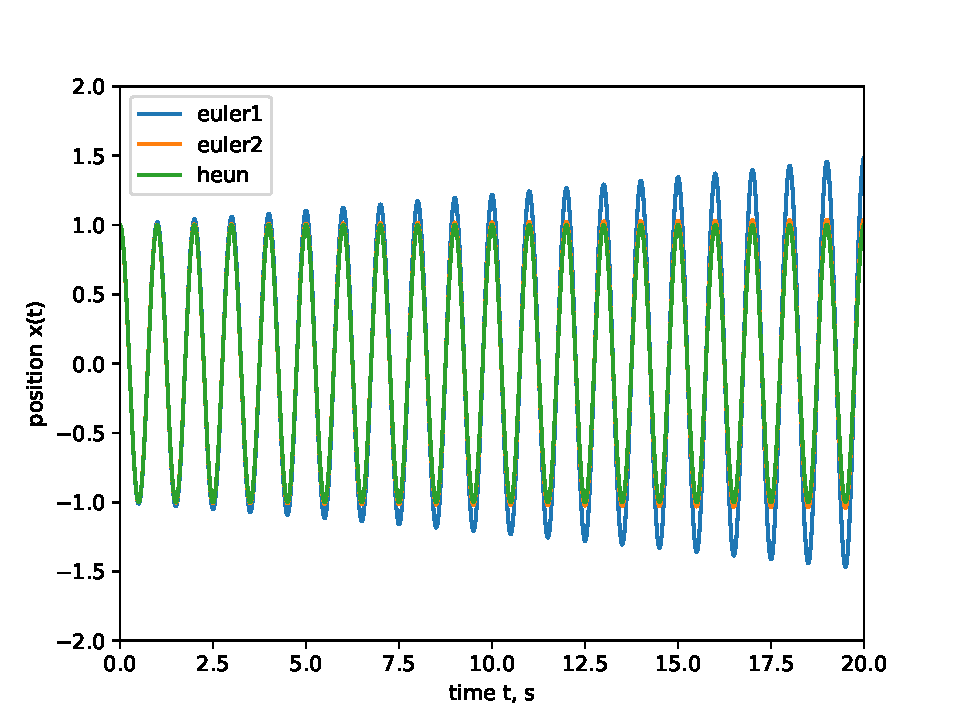
\includegraphics[width=\textwidth]{figures/eul12+heun.pdf}
			\caption{Position as a funcion of time. Notice how eul1 deviates very fast.\label{subfig:sho-pos}}
		\end{subfigure}
		\hfill
		\begin{subfigure}[t]{0.48\textwidth}
			\centering
			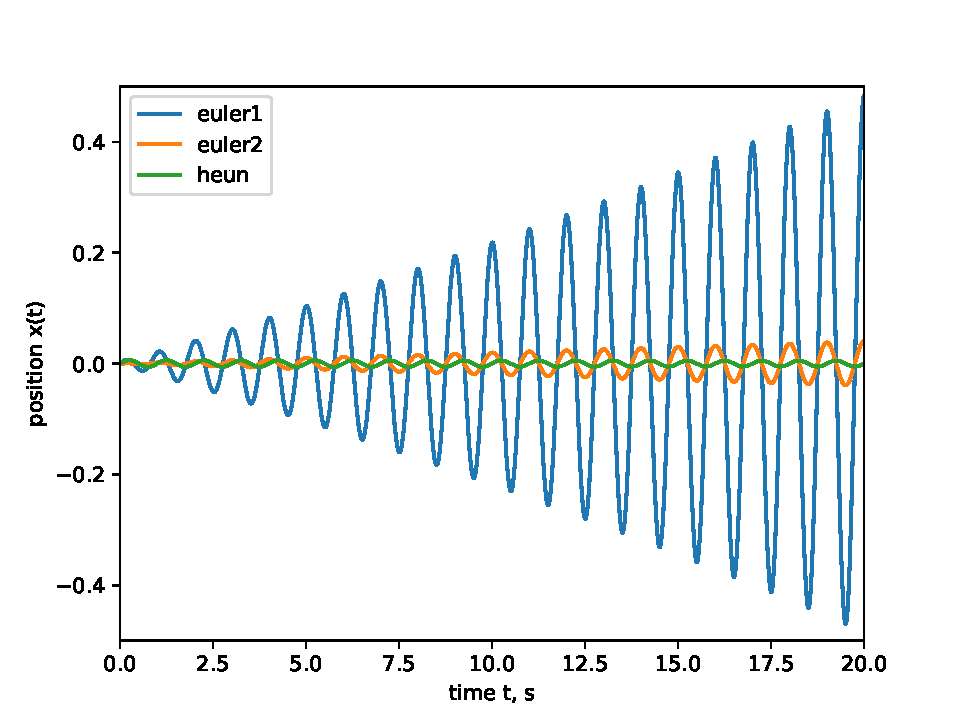
\includegraphics[width=\textwidth]{figures/eul12+heun-theory.pdf}
			\caption{Deviation from the theoretical solution.\label{subfig:sho-dev}}
		\end{subfigure}
		\hfill

		\hfill
		\begin{subfigure}[t]{0.48\textwidth}
			\centering
			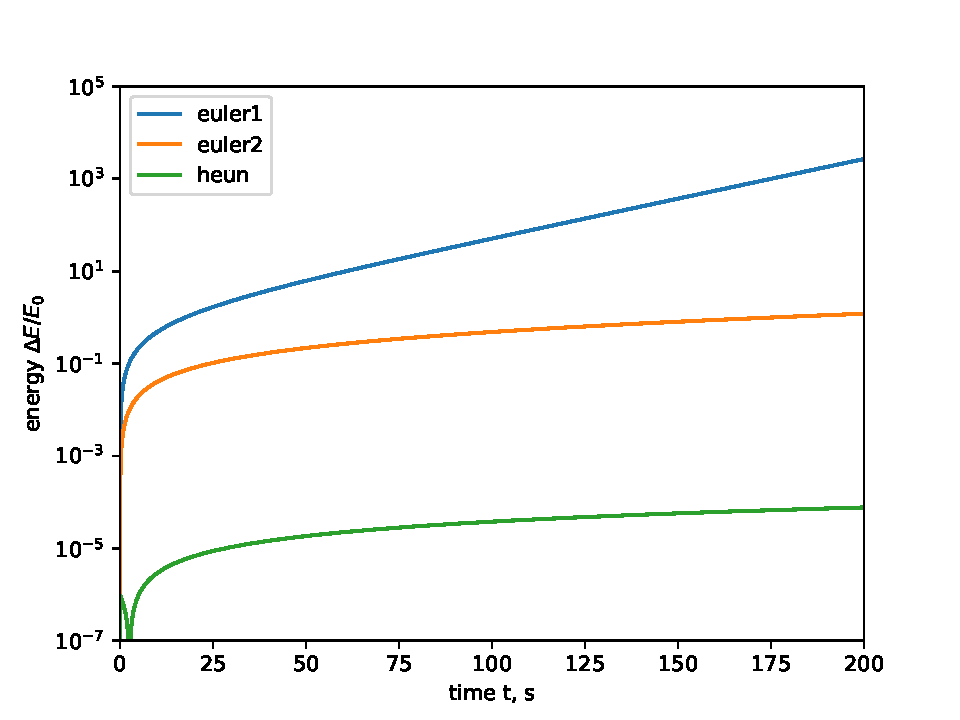
\includegraphics[width=\textwidth]{figures/eul12+heun+energy.pdf}
			\caption{Energy deviation $\Delta E/E_0$ for first three methods.\label{subfig:sho-energy1}}
		\end{subfigure}
		\hfill
		\begin{subfigure}[t]{0.48\textwidth}
			\centering
			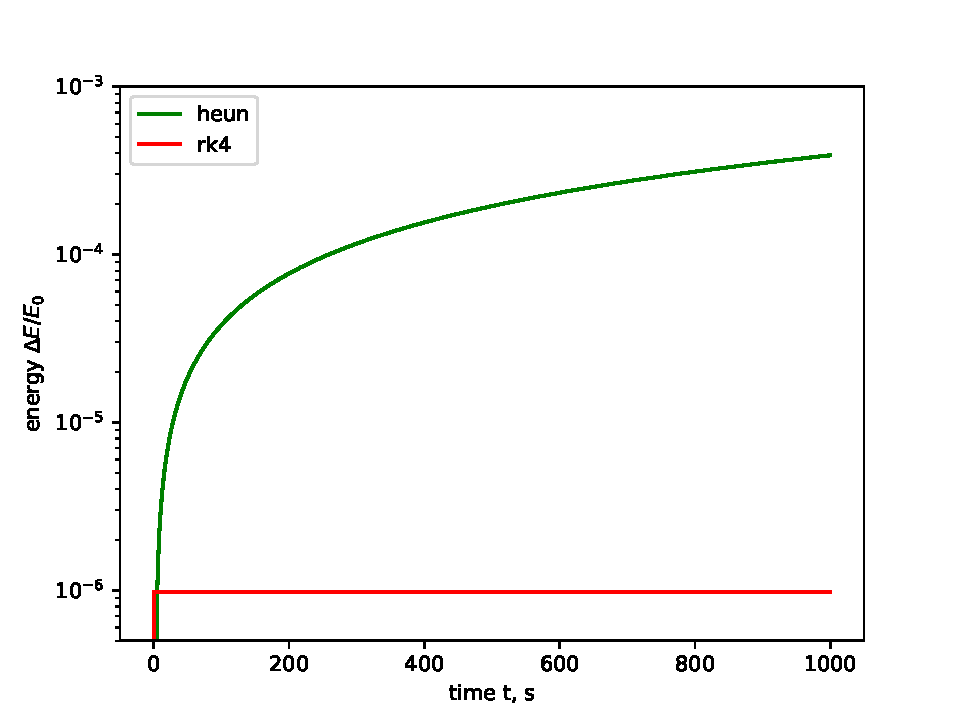
\includegraphics[width=\textwidth]{figures/heunRK4+energy.pdf}
			\caption{Energy deviation $\Delta E/E_0$ for heun and rk4.\label{subfig:sho-energy2}}
		\end{subfigure}
		\hfill
		\caption{Test runs of SHO integrated with different methods. Blue line is for Euler's method integrated with step \SI{1}{ms}, yellow line for Euler's method integrated with step \SI{0.1}{ms}, green line is for Heun's method with step \SI{1}{ms}, and red line is for RK4 method with step \SI{1}{ms}.\label{fig:sho-integration}}
	\end{figure}

	With these results in mind, we make the obvious choice for a method and continute forwards using the Runge-Kutta 4th order method in all of the following chapters.


\subsection{Dimensionless equation for the white dwarf}
	%		- Normalization - take into form that is implemented in the program
	To calculate values with the compute, we will go to dimensionless quantities in the differential equation. Introduce the following substitutions:
	\begin{equation}
		\rho = \rhoCentre \theta, \quad r = \ell \xi, \quad m = \rhoCentre (\SI{1}{m^3}) \mu
	\end{equation}
	where we chage variables from $\vec{y}(r) = \begin{pmatrix}\rho(r) \\ m(r)\end{pmatrix}$ to $\vec{\eta}(\xi) = \begin{pmatrix}\theta(\xi)\\\mu(\xi)\end{pmatrix}$. We also specify the length $\ell$ by the equation $\frac{4}{3}\pi \ell^3 = \SI{1}{m^3}$, which gives a value of $\ell \approx 0.62 \sim \SI{1}{m}$. This will be useful to make some cancelations in the coefficients in the final form of the differential equation for $\vec{\eta}$.

	For \eqref{eqn:mass-dEq}  the conversion is straightforward:
	\begin{equation}
		\frac{\rhoCentre \dd \mu}{\ell \dd \xi} = 4 \pi \ell^2 \xi^2 \rhoCentre \theta \quad \Rightarrow \quad \frac{\dd \mu}{\dd \xi} = 3 \xi^2 \theta.
	\end{equation}

	For the $\theta$ equation we have to take into consideration the regime we operate in --- whether we solve for a relativistic or non-relativistic equation of state. Firstly, write equations in \eqref{eqn:fermi-mtm} using the new coordinates we have introduced:
	\begin{equation}\label{eqn:fermi-mtm-new}
		\fermiMtm = \left( \frac{h^3 \rhoCentre}{16 \pi \massProton}\right)^{\sfrac{1}{3}} \theta^{\sfrac{1}{3}} , \quad \frac{\dd \fermiMtm}{\dd \rho} = \frac{1}{3} \left( \frac{h^3}{16 \pi \massProton \rhoCentre^2}\right)^{\sfrac{1}{3}} \theta^{-\sfrac{2}{3}}.
	\end{equation}
	Now substitute \eqref{eqn:pressure-both} in \eqref{eqn:hydrostat-equil-rhor} using \eqref{eqn:fermi-mtm-new}. After some algebra with the constants, the final result is the following:
	\begin{equation}
		\frac{\dd \theta}{\dd \xi} = K_1 \frac{\mu \theta^{\sfrac{1}{3}}}{\xi^2} \begin{cases}
			1 & \text{ in the non-relativistic case}\\
			\left(1 + K_2 \theta^{\sfrac{2}{3}}\right)^{\sfrac{1}{2}} & \text{ in the relativistic case}
		\end{cases},
	\end{equation}
	where the constants $K_1$ and $K_2$ are given by
	\begin{equation}
		K_1 = - 2^{\sfrac{13}{3}} \pi \gravconst \massElectron \massProton^{\sfrac{5}{3}} \rhoCentre^{\sfrac{1}{3}} h^{-2} , \quad \quad K_2 = \frac{1}{\massElectron^2 c^2} \left( \frac{3h^3 \rhoCentre}{16 \pi \massProton} \right)^{\sfrac{2}{3}}.
	\end{equation}
	We have completed the task of bringing the equation to normalized coordinates. 

\subsection{Convergence and iterations}\label{subsec:convergence}
	%		- Convergence => determine number of steps
	What is left is to choose the coarsness in the grid of $\xi$. We know that for some $\Delta \xi$ small enough, the answers will converge to $\approx$ a single value. To do this, we will make several experimental runs at three different $\rhoCentre$ --- $10$ Test this by experimental runs at three different central densities --- two at the end of the interval and 1 in the middle.

\section{Results and discussion}\label{sec:results-and-discussion}
%Section 4 - Results and discussion
%		- state how much of the parameter space was studied
%		- R(rhoC)
%		- mass(rhoC)
%		- R(mass) and the Chandrasekhar limit
%		-- discuss the results and their implications about nature of white dwarfs, relation to stellar evolution i.e. implications of the limit, relation to other compact objects neutron stars/BHs.


\section{Summary}\label{sec:summary}
this is a citation \cite{Sagert2005}
%Section 5 - Summary
%		- present task, method, and result
%		- propose directions of improvement on:
%			- numerical approach
%			- physics of white dwarfs

% References - placeholder for noу
\bibliographystyle{agsm}
\renewcommand{\bibname}{References}
\bibliography{test}

% \begin{thebibliography}{9}
	
% 	\bibitem{labscript}
% 	Various,
% 	\textit{OP14: Fraunhofer diffraction},
% 	Oxford Physics,
% 	January 2019.	
	
% 	\bibitem{chandrasekhar-white-dwarf}
% 	Chandrasekhar S.,
% 	\textit{Sth},
% 	Publication,
% 	Year.

% 	\bibitem{eso-vlt}
% 	Richard J, Bacon R, et al.
% 	\textit{MUSE User Manual},
% 	Document Version 11.3,
% 	"\url{http://www.eso.org/sci/facilities/paranal/instruments/muse/doc.html}"
% 	December 2019.
	
% 	\bibitem{hecht}
% 	Hecht E,
% 	\textit{Optics},
% 	Addison-Wesley, Massachusetts,
% 	4th edition (international),
% 	2002.
	
% 	\bibitem{experim-err}
% 	Various,
% 	\textit{Estimating experimental errors},
% 	Oxford Physics,
% 	August 2011.
	
% \end{thebibliography}

\appendix
\section{Source code}\label{app:source-code}
%Appendix A - source code
\section{Derivations of white dwarf}\label{app:WD-derivations}
%Appendix B - theory derivation of white dwarf concrete formulae

\end{document}